% titlepage-demo.tex
\documentclass{beamer}
\usepackage{graphicx}
\usepackage{tikz}
\usetikzlibrary{matrix}
% items enclosed in square brackets are optional; explanation below
\title{Verifying filesystems in ACL2}
\subtitle{Towards verifying file recovery tools}
\author{Mihir Mehta}
\institute{
  Department of Computer Science\\
  University of Texas at Austin\\[1ex]
  \texttt{mihir@cs.utexas.edu}
}
\date{10 November, 2017}

\AtBeginSection[]
{
  \begin{frame}<beamer>
    \frametitle{Outline}
    \tableofcontents[currentsection]
  \end{frame}
}

\addtobeamertemplate{navigation symbols}{}{%
    \usebeamerfont{footline}%
    \usebeamercolor[fg]{footline}%
    \hspace{1em}%
    \large \insertframenumber/\inserttotalframenumber
}

\begin{document}

%--- the titlepage frame -------------------------%
\begin{frame}[plain]
  \titlepage
\end{frame}

%--- the presentation begins here ----------------%

\section{Motivation and related work}

\begin{frame}{Why we need a verified filesystem}
  \begin{itemize}
  \item Filesystems are everywhere, even as operating systems move
    towards making them invisible.
  \item In the absence of a clear specification of filesystems, users
    (and sysadmins in particular) are underserved.
  \item Modern filesystems have become increasingly complex, and so
    have the tools to analyse and recover data from them.
  \item It would be worthwhile to specify and formally verify, in the
    ACL2 theorem prover, the guarantees claimed by filesystems and tools.
  \end{itemize}
\end{frame}

\begin{frame}{Related work}
  \begin{itemize}
  \item In Haogang Chen's 2016 dissertation, the author uses Coq to
    build a filesystem (named FSCQ) which is proven safe against
    crashes in a new logical framework named Crash Hoare Logic. His
    (exported) Haskell implementation performs comparably to ext4.
  \item Hyperkernel (Nelson et al., SOSP '17) is a "push-button"
    verification effort, but approximates by changing POSIX system
    calls for ease of verification.
  \item In our work, we instead aim to model an existing filesystem (FAT32)
    faithfully and match the resulting disk image byte-to-byte.
  \end{itemize}
\end{frame}

\section{Our approach}

\begin{frame}{File system models}
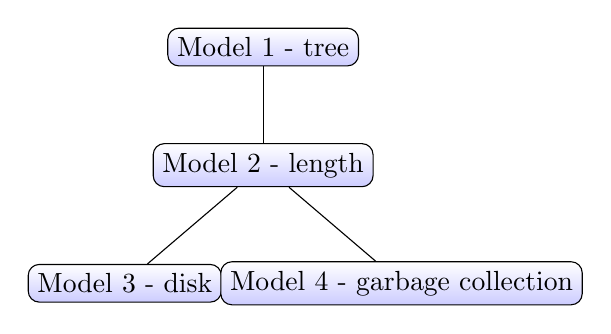
\begin{tikzpicture}[sibling distance=10em,
  every node/.style = {shape=rectangle, rounded corners,
    draw, align=center,
    top color=white, bottom color=blue!20}]
  \node {Model 1 - tree}
    child { node {Model 2 - length}
      child { node {Model 3 - disk}}
      child { node {Model 4 - garbage collection}}};
\end{tikzpicture}
\end{frame}

\begin{frame}{Choosing an initial model}
  \begin{itemize}
    \item Our goal here is to verify the FAT32 filesystem, but we need
      a simpler model to begin with.
    \item Our filesystem's operations should suffice for running a
      workload.
    \item Yet, parsimony and avoidance of redundancy are helpful for
      theorem proving.
    \item What's a necessary and sufficient set of operations?
  \end{itemize}
\end{frame}

%% \begin{frame}[fragile]
%% \begin{verbatim}
%% struct inode_operations {
%%         int (*create) (struct inode *, struct dentry *, int);
%%         struct dentry * (*lookup) (struct inode *, struct dentry *);
%%         int (*link) (struct dentry *, struct inode *, struct dentry *);
%%         int (*unlink) (struct inode *, struct dentry *);
%%         int (*symlink) (struct inode *, struct dentry *, const char *);
%%         int (*mkdir) (struct inode *, struct dentry *, int);
%%         int (*rmdir) (struct inode *, struct dentry *);
%%         int (*mknod) (struct inode *, struct dentry *, int, dev_t);
%%         int (*rename) (struct inode *, struct dentry *, struct inode *, struct dentry *);
%%         int (*readlink) (struct dentry *, char *,int);
%%         int (*follow_link) (struct dentry *, struct nameidata *);
%%         void (*truncate) (struct inode *);
%%         int (*permission) (struct inode *, int);
%%         int (*setattr) (struct dentry *, struct iattr *);
%%         int (*getattr) (struct vfsmount *mnt, struct dentry *, struct kstat *);
%%         int (*setxattr) (struct dentry *, const char *, const void *, size_t, int);
%%         ssize_t (*getxattr) (struct dentry *, const char *, void *, size_t);
%%         ssize_t (*listxattr) (struct dentry *, char *, size_t);
%%         int (*removexattr) (struct dentry *, const char *);
%% };
%% \end{verbatim}
%% \end{frame}

\begin{frame}{Minimal set of operations?}
  \begin{itemize}
  \item The Google filesystem suggests a minimal set of operations:
    \begin{itemize}
    \item \texttt{create}
    \item \texttt{delete}
    \item \texttt{open}
    \item \texttt{close}
    \item \texttt{read}
    \item \texttt{write}
    \end{itemize}
  \item Of these, \texttt{open} and \texttt{close} require the
    maintenance of file descriptor state - so they can wait.
  \item However, they are essential when describing concurrency and
    multiprogramming behaviour.
  \item Thus, we can start modelling a filesystem, and several
    refinements thereof.
  \end{itemize}
\end{frame}

\begin{frame}{Quick overview of models}
  \begin{itemize}
  \item What follows is a sequence of {\bf increasingly refined} models.
  \item Model 1: Tree representation of directory structure with unbounded
    file size and unbounded filesystem size.
  \item Model 2: Model 1 with file length as metadata.
  \item Model 3: Tree representation of directory structure with
    file contents stored in a "disk" (unbounded in length).
  \item Model 4: Model 3 with bounded filesystem size and garbage
    collection.
  \item In our running example, we'll observe file creation, deletion,
    and overwriting in each of these models in turn.
  \end{itemize}
\end{frame}

\begin{frame}{Model 1}
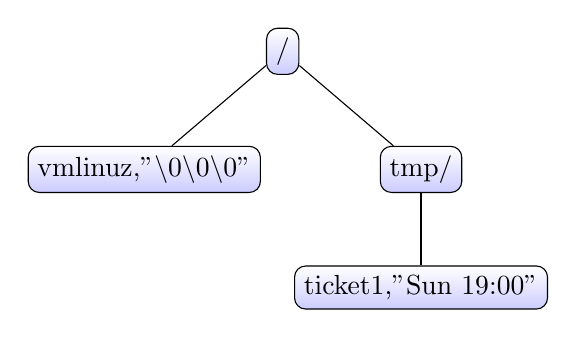
\begin{tikzpicture}[sibling distance=10em,
  every node/.style = {shape=rectangle, rounded corners,
    draw, align=center,
    top color=white, bottom color=blue!20}]
  \node {/}
    child { node {vmlinuz,{"}\textbackslash0\textbackslash0\textbackslash0{"}} }
    child { node {tmp/}
      child { node {ticket1,{"}Sun 19:00{"}}}};
\end{tikzpicture}
\end{frame}

\begin{frame}{Model 1}
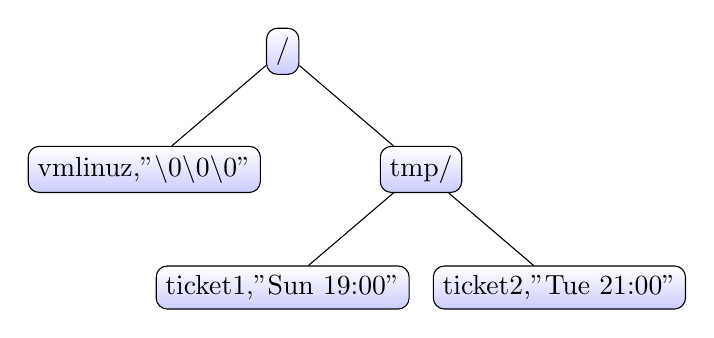
\begin{tikzpicture}[sibling distance=10em,
  every node/.style = {shape=rectangle, rounded corners,
    draw, align=center,
    top color=white, bottom color=blue!20}]
  \node {/}
    child { node {vmlinuz,{"}\textbackslash0\textbackslash0\textbackslash0{"}} }
    child { node {tmp/}
      child { node {ticket1,{"}Sun 19:00{"}}}
      child { node {ticket2,{"}Tue 21:00{"}}}};
\end{tikzpicture}
\end{frame}

\begin{frame}{Model 1}
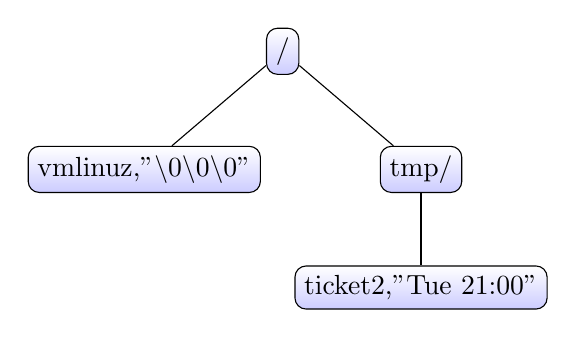
\begin{tikzpicture}[sibling distance=10em,
  every node/.style = {shape=rectangle, rounded corners,
    draw, align=center,
    top color=white, bottom color=blue!20}]
  \node {/}
    child { node {vmlinuz,{"}\textbackslash0\textbackslash0\textbackslash0{"}} }
    child { node {tmp/}
      child { node {ticket2,{"}Tue 21:00{"}}}};
\end{tikzpicture}
\end{frame}

\begin{frame}{Model 1}
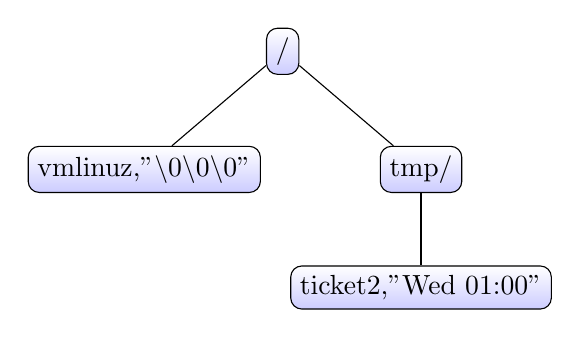
\begin{tikzpicture}[sibling distance=10em,
  every node/.style = {shape=rectangle, rounded corners,
    draw, align=center,
    top color=white, bottom color=blue!20}]
  \node {/}
    child { node {vmlinuz,{"}\textbackslash0\textbackslash0\textbackslash0{"}} }
    child { node {tmp/}
      child { node {ticket2,{"}Wed 01:00{"}}}};
\end{tikzpicture}
\end{frame}

\begin{frame}{Model 2}
  \begin{itemize}
  \item Model 1 supports nested directory structures, unbounded file
    size and unbounded filesystem size.
  \item However, there's no metadata, either to provide additional
    information or to validate the contents of the file.
  \item With an extra field for length, we can create a simple
    version of fsck that checks file contents for consistency.
  \item Further, we can verify that create, write, delete etc preserve
    this notion of consistency.
  \end{itemize}
\end{frame}

\begin{frame}{Model 2}
  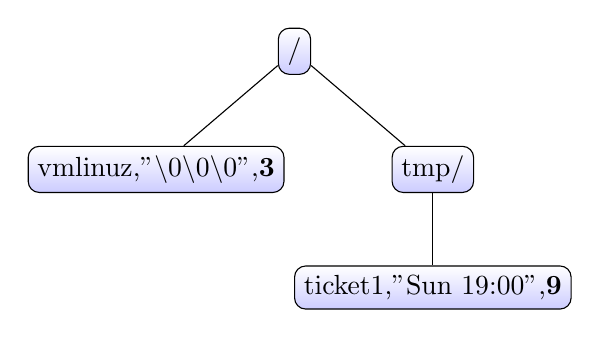
\begin{tikzpicture}[sibling distance=10em,
      every node/.style = {shape=rectangle, rounded corners,
        draw, align=center,
        top color=white, bottom color=blue!20}]]
      \node {/}
      child { node {vmlinuz,{"}\textbackslash0\textbackslash0\textbackslash0{"},{\bf 3}} }
      child { node {tmp/}
        child { node {ticket1,{"}Sun 19:00{"},{\bf 9}}}};
  \end{tikzpicture}
\end{frame}

\begin{frame}{Model 2}
  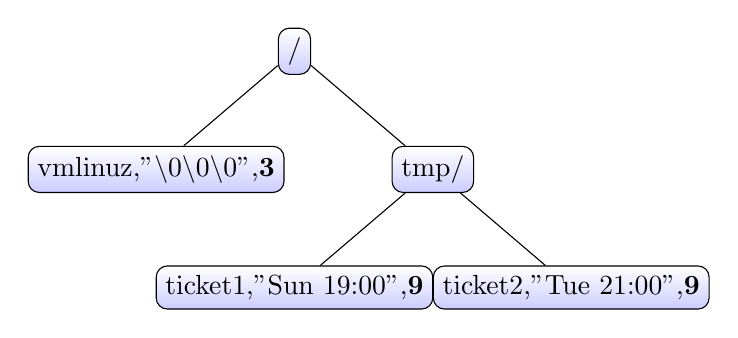
\begin{tikzpicture}[sibling distance=10em,
      every node/.style = {shape=rectangle, rounded corners,
        draw, align=center,
        top color=white, bottom color=blue!20}]]
      \node {/}
      child { node {vmlinuz,{"}\textbackslash0\textbackslash0\textbackslash0{"},{\bf 3}} }
      child { node {tmp/}
        child { node {ticket1,{"}Sun 19:00{"},{\bf 9}}}
        child { node {ticket2,{"}Tue 21:00{"},{\bf 9}}}};
  \end{tikzpicture}
\end{frame}

\begin{frame}{Model 2}
  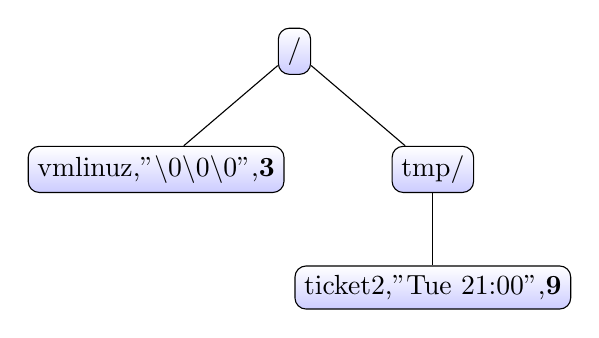
\begin{tikzpicture}[sibling distance=10em,
      every node/.style = {shape=rectangle, rounded corners,
        draw, align=center,
        top color=white, bottom color=blue!20}]]
      \node {/}
      child { node {vmlinuz,{"}\textbackslash0\textbackslash0\textbackslash0{"},{\bf 3}} }
      child { node {tmp/}
        child { node {ticket2,{"}Tue 21:00{"},{\bf 9}}}};
  \end{tikzpicture}
\end{frame}

\begin{frame}{Model 2}
  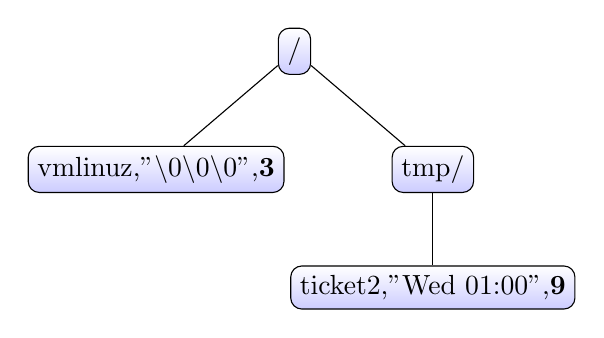
\begin{tikzpicture}[sibling distance=10em,
      every node/.style = {shape=rectangle, rounded corners,
        draw, align=center,
        top color=white, bottom color=blue!20}]]
      \node {/}
      child { node {vmlinuz,{"}\textbackslash0\textbackslash0\textbackslash0{"},{\bf 3}} }
      child { node {tmp/}
        child { node {ticket2,{"}Wed 01:00{"},{\bf 9}}}};
  \end{tikzpicture}
\end{frame}

\begin{frame}{Model 3}
  \begin{itemize}
  \item As the next step, we focus on externalising the
    storage of file contents.
  \item We also choose to break up file contents into "blocks"
    of a constant length (8).
    \begin{itemize}
    \item Note: this would mean storing file length is no longer
      optional, to avoid reading garbage past end of file at the end
      of a block.
    \end{itemize}
  \end{itemize}
\end{frame}

\begin{frame}{Model 3}
  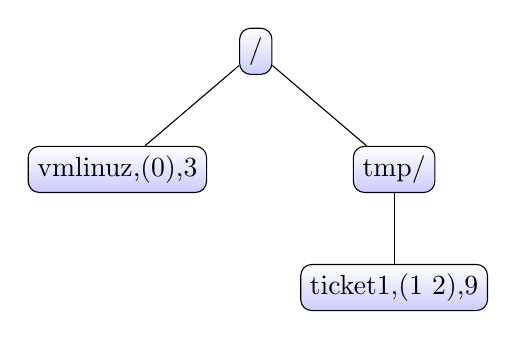
\begin{tikzpicture}[sibling distance=10em,
      every node/.style = {shape=rectangle, rounded corners,
        draw, align=center,
        top color=white, bottom color=blue!20}]]
      \node {/}
      child { node {vmlinuz,(0),3} }
      child { node {tmp/}
        child { node {ticket1,(1 2),9}}};
  \end{tikzpicture}
  \begin{table}[]
    %% \centering
    \caption{Disk}
    % \label{my-label}
    \begin{tabular}{|l|l|}
      \hline
      0 & \textbackslash0\textbackslash0\textbackslash0   \\ \hline
      1 & Sun 19:0 \\ \hline
      2 & 0        \\ \hline
    \end{tabular}
  \end{table}
\end{frame}

\begin{frame}{Model 3}
  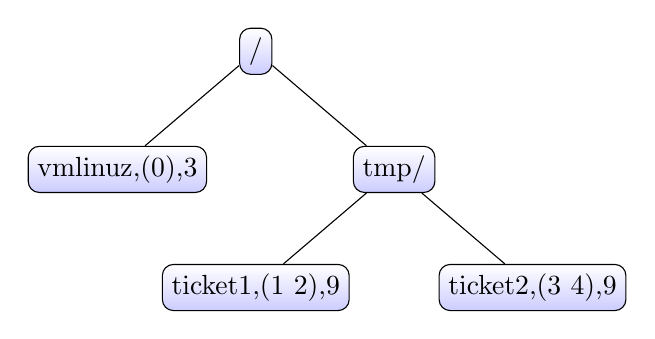
\begin{tikzpicture}[sibling distance=10em,
      every node/.style = {shape=rectangle, rounded corners,
        draw, align=center,
        top color=white, bottom color=blue!20}]]
      \node {/}
      child { node {vmlinuz,(0),3} }
      child { node {tmp/}
        child { node {ticket1,(1 2),9}}
        child { node {ticket2,(3 4),9}}};
  \end{tikzpicture}
  \begin{table}[]
    \centering
    \caption{Disk}
    % \label{my-label}
    \begin{tabular}{|l|l|}
      \hline
      0 & \textbackslash0\textbackslash0\textbackslash0   \\ \hline
      1 & Sun 19:0 \\ \hline
      2 & 0        \\ \hline
      3 & Tue 21:0 \\ \hline
      4 & 0        \\ \hline
    \end{tabular}
  \end{table}
\end{frame}

\begin{frame}{Model 3}
  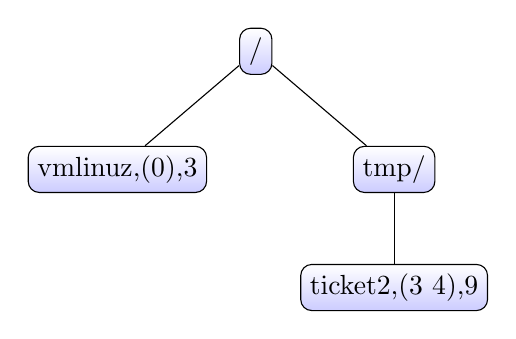
\begin{tikzpicture}[sibling distance=10em,
      every node/.style = {shape=rectangle, rounded corners,
        draw, align=center,
        top color=white, bottom color=blue!20}]]
      \node {/}
      child { node {vmlinuz,(0),3} }
      child { node {tmp/}
        child { node {ticket2,(3 4),9}}};
  \end{tikzpicture}
  \begin{table}[]
    \centering
    \caption{Disk}
    % \label{my-label}
    \begin{tabular}{|l|l|}
      \hline
      0 & \textbackslash0\textbackslash0\textbackslash0   \\ \hline
      1 & Sun 19:0 \\ \hline
      2 & 0        \\ \hline
      3 & Tue 21:0 \\ \hline
      4 & 0        \\ \hline
    \end{tabular}
  \end{table}
\end{frame}

\begin{frame}{Model 3}
  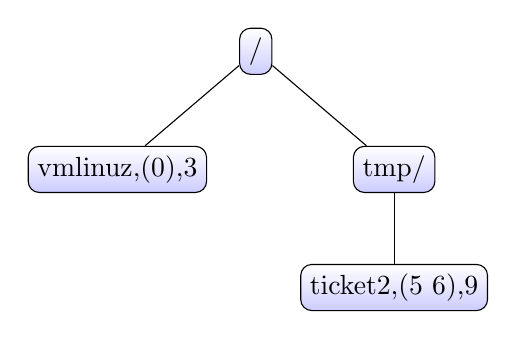
\begin{tikzpicture}[sibling distance=10em,
      every node/.style = {shape=rectangle, rounded corners,
        draw, align=center,
        top color=white, bottom color=blue!20}]]
      \node {/}
      child { node {vmlinuz,(0),3} }
      child { node {tmp/}
        child { node {ticket2,(5 6),9}}};
  \end{tikzpicture}
  \begin{table}[]
    \centering
    \caption{Disk}
    % \label{my-label}
    \begin{tabular}{|l|l|}
      \hline
      0 & \textbackslash0\textbackslash0\textbackslash0   \\ \hline
      1 & Sun 19:0 \\ \hline
      2 & 0        \\ \hline
      3 & Tue 21:0 \\ \hline
      4 & 0        \\ \hline
      5 & Wed 01:0 \\ \hline
      6 & 0        \\ \hline
    \end{tabular}
  \end{table}
\end{frame}

\begin{frame}{Model 4}
  \begin{itemize}
  \item In the fourth model, we attempt to implement garbage
    collection in the form of an allocation vector.
  \item The allocation vector tracks whether blocks in the filesystem
    are in use by a file. This allows us to reuse unused blocks.
  \end{itemize}
\end{frame}

\begin{frame}{Model 4}
  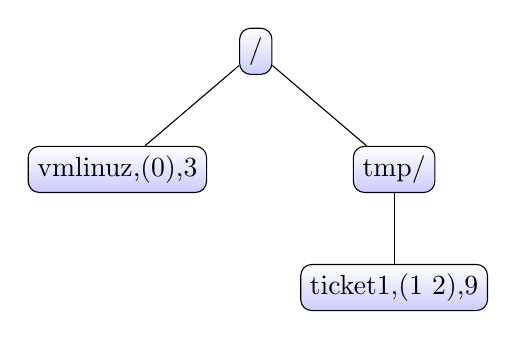
\begin{tikzpicture}[sibling distance=10em,
      every node/.style = {shape=rectangle, rounded corners,
        draw, align=center,
        top color=white, bottom color=blue!20}]]
      \node {/}
      child { node {vmlinuz,(0),3} }
      child { node {tmp/}
        child { node {ticket1,(1 2),9}}};
  \end{tikzpicture}
  \begin{table}[]
    %% \centering
    \caption{Disk and allocation vector}
    \begin{tabular}{|l|l|l|}
      \hline
      0 & \textbackslash0\textbackslash0\textbackslash0   & true\\ \hline
      1 & Sun 19:0 & true\\ \hline
      2 & 0        & true\\ \hline
      3 &          & false\\ \hline
      4 &          & false\\ \hline
      5 &          & false\\ \hline
    \end{tabular}
  \end{table}
\end{frame}

\begin{frame}{Model 4}
  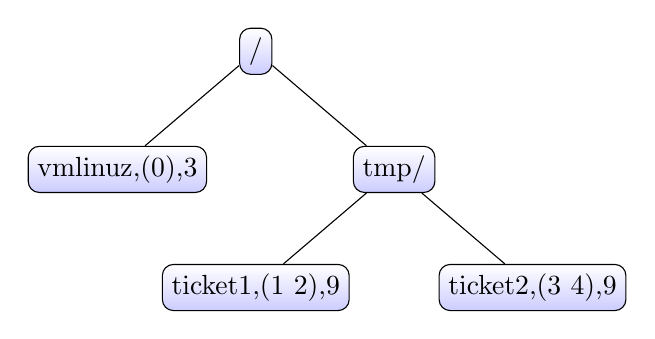
\begin{tikzpicture}[sibling distance=10em,
      every node/.style = {shape=rectangle, rounded corners,
        draw, align=center,
        top color=white, bottom color=blue!20}]]
      \node {/}
      child { node {vmlinuz,(0),3} }
      child { node {tmp/}
        child { node {ticket1,(1 2),9}}
        child { node {ticket2,(3 4),9}}};
  \end{tikzpicture}
  \begin{table}[]
    \centering
    \caption{Disk and allocation vector}
    \begin{tabular}{|l|l|l|}
      \hline
      0 & \textbackslash0\textbackslash0\textbackslash0   & true\\ \hline
      1 & Sun 19:0 & true\\ \hline
      2 & 0        & true\\ \hline
      3 & Tue 21:0 & true\\ \hline
      4 & 0        & true\\ \hline
      5 &          & false\\ \hline
    \end{tabular}
  \end{table}
\end{frame}

\begin{frame}{Model 4}
  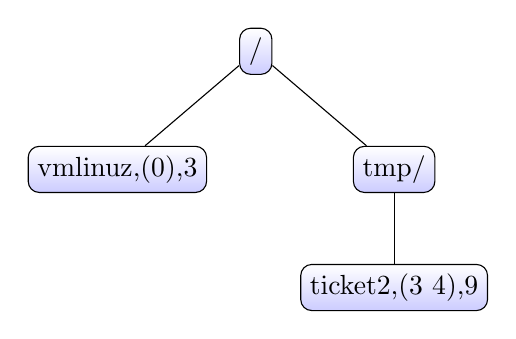
\begin{tikzpicture}[sibling distance=10em,
      every node/.style = {shape=rectangle, rounded corners,
        draw, align=center,
        top color=white, bottom color=blue!20}]]
      \node {/}
      child { node {vmlinuz,(0),3} }
      child { node {tmp/}
        child { node {ticket2,(3 4),9}}};
  \end{tikzpicture}
  \begin{table}[]
    \centering
    \caption{Disk and allocation vector}
    \begin{tabular}{|l|l|l|}
      \hline
      0 & \textbackslash0\textbackslash0\textbackslash0   & true\\ \hline
      1 & Sun 19:0 & false\\ \hline
      2 & 0        & false\\ \hline
      3 & Tue 21:0 & true\\ \hline
      4 & 0        & true\\ \hline
      5 &          & false\\ \hline
    \end{tabular}
  \end{table}
\end{frame}

\begin{frame}{Model 4}
  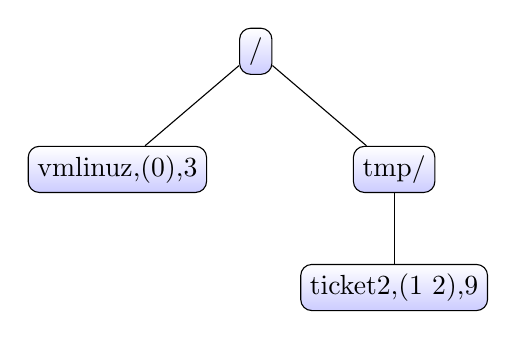
\begin{tikzpicture}[sibling distance=10em,
      every node/.style = {shape=rectangle, rounded corners,
        draw, align=center,
        top color=white, bottom color=blue!20}]]
      \node {/}
      child { node {vmlinuz,(0),3} }
      child { node {tmp/}
        child { node {ticket2,(1 2),9}}};
  \end{tikzpicture}
  \begin{table}[]
    \centering
    \caption{Disk and allocation vector}
    \begin{tabular}{|l|l|l|}
      \hline
      0 & \textbackslash0\textbackslash0\textbackslash0   & true\\ \hline
      1 & Wed 01:0 & true\\ \hline
      2 & 0        & true\\ \hline
      3 & Tue 21:0 & false\\ \hline
      4 & 0        & false\\ \hline
      5 &          & false\\ \hline
    \end{tabular}
  \end{table}
\end{frame}

\section{Progress so far}
\begin{frame}{Proof approaches and techniques}
  \begin{itemize}
  \item There are many properties that could be considered for
    correctness, but we choose to focus on the read-over-write
    theorems from the first-order theory of arrays.
  \item Read \texttt{n} characters starting at position \texttt{start}
    in the file at path \texttt{hns} in filesystem \texttt{fs}: \\
    \texttt{l1-rdchs(hns, fs, start, n)}
  \item Write string \texttt{text} characters starting at position \texttt{start}
    in the file at path \texttt{hns} in filesystem \texttt{fs}: \\
    \texttt{l1-wrchs(hns, fs, start, text)}
  \end{itemize}
\end{frame}
\begin{frame}{Proof approaches and techniques}
  \begin{itemize}
  \item First read-over-write theorem: reading from a location after writing to the same location
    should yield the data that was written. Formally, assuming \texttt{n =
      length(text)} and suitable "type" hypotheses (omitted here): \\
    \texttt{l1-rdchs(hns, l1-wrchs(hns, fs, start, text), start, n) \\
      = \\
      text}
  \item Second read-over-write-theorem: Reading from a location after writing to a different
    location should yield the same result as reading before
    writing. Formally, assuming \texttt{hns1 != hns2} and suitable "type"
    hypotheses (omitted here):\\
    \texttt{l1-rdchs(hns1, l1-wrchs(hns2, fs, start2, text2), start1, n1) \\
      = \\
      l1-rdchs(hns1, fs, start1, n1)}
  \end{itemize}
\end{frame}

\begin{frame}{Proof approaches and techniques}
  \begin{itemize}
  \item For each of the models 1, 2, 3 and 4, we have proofs of correctness of
    the two read-after-write properties, making use of the proofs of
    equivalence between models and their successors.
  \item Model 4 presented some unique challenges - proving the
    read-after-write properties required proving an equivalence
    between model 4 and model 2, rather than model 3.
  \end{itemize}
\end{frame}

\begin{frame}{Proof approaches and techniques}
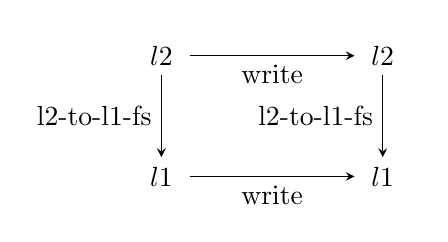
\begin{tikzpicture}
  \matrix (m) [matrix of math nodes,row sep=3em,column sep=6em,minimum width=2em]
  {
     l2 \pgfmatrixnextcell l2 \\
     l1 \pgfmatrixnextcell l1 \\};
  \path[-stealth]
    (m-1-1) edge node [left] {l2-to-l1-fs} (m-2-1)
            edge node [below] {write} (m-1-2)
    (m-2-1.east|-m-2-2) edge node [below] {write} (m-2-2)
    (m-1-2) edge node [left] {l2-to-l1-fs} (m-2-2);
\end{tikzpicture}
\begin{tikzpicture}
  \matrix (m) [matrix of math nodes,row sep=3em,column sep=6em,minimum width=2em]
  {
     l2 \pgfmatrixnextcell text \\
     l1 \\};
  \path[-stealth]
    (m-1-1) edge node [left] {l2-to-l1-fs} (m-2-1)
            edge node [below] {read} (m-1-2)
    (m-2-1.east|-m-2-2) edge node [below] {read} (m-1-2);
\end{tikzpicture}
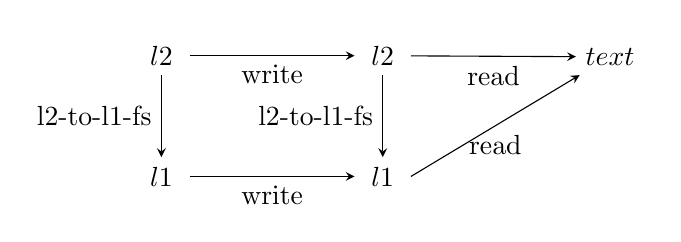
\begin{tikzpicture}
  \matrix (m) [matrix of math nodes,row sep=3em,column sep=6em,minimum width=2em]
  {
     l2 \pgfmatrixnextcell l2 \pgfmatrixnextcell text \\
     l1 \pgfmatrixnextcell l1 \\};
  \path[-stealth]
    (m-1-1) edge node [left] {l2-to-l1-fs} (m-2-1)
            edge node [below] {write} (m-1-2)
    (m-2-1.east|-m-2-2) edge node [below] {write} (m-2-2)
    (m-1-2) edge node [left] {l2-to-l1-fs} (m-2-2)
            edge node [below] {read} (m-1-3)
    (m-2-2.east) edge node [below] {read} (m-1-3);
\end{tikzpicture}
\end{frame}

\begin{frame}{Source analysis}
  \begin{table}[]
    \centering
    \caption{Code (over ~3 semesters)}
    \label{my-label}
    \begin{tabular}{ll}
      sloccount (lines of ACL2 code)      & 4964 \\
      defun events (function definitions) & 106  \\
      defthm events (lemmas and proofs)   & 374 
    \end{tabular}
  \end{table}
\end{frame}

\section{Future work}

\begin{frame}{Future work}
  \begin{itemize}
  \item Model and verify file permissions.
  \item Linearise the tree, leaving only the disk.
  \item Add the system call open and close with the
    introduction of file descriptors.\\
    \textit{This would be a step towards the study of concurrent FS operations.}
  \item Eventually emulate the FAT32 filesystem as a convincing proof
    of concept, and move on to fsck and file recovery tools.
  \end{itemize}
\end{frame}

\end{document}
